\setauthor{Isabel Schnalzenberger}

\section{Technologien}

\subsection{Angular}

\textbf{Angular}\footnote{Alle hier stehenden Informationen zum Projekt stammen von \cite{Angular}} ist ein Open-Source-Webanwendungs-Framework, das von Google laufend (weiter-)entwickelt wird. Es wird vor allem für die Erstellung von \Glspl{spa} verwendet und bietet eine strukturierte Lösung für die Entwicklung von dynamischen und komplexen Webanwendungen. Angular basiert auf \textbf{TypeScript}, einer streng typisierten Variante von JavaScript, was eine verbesserte Codequalität und Wartbarkeit ermöglicht.

Die Entwickler haben sich aufgrund der erworbenen, gemeinsamen Kenntnisse in Typescript und Angular für diese Technologie entschieden. Die gebotenen Funktionen rund um \emph{Datenbindung}, Dependency Injection und \emph{Routing} können die Anforderungen an das Memoryland Frontend erfüllen. Zusätzlich bietet die enge Integration mit TypeScript und seiner starken Community, die es zu einem der beliebtesten Frameworks für die Frontend-Entwicklung machen, viele Quellen für mögliche Unterstützung während der Entwicklung.


\subsection{Bootstrap}

Auch \textbf{Bootstrap}\footnote{Alle hier stehenden Informationen zum Projekt stammen von \cite{Bootstrap}}  ist ein beliebtes Open-Source Frontend-Framework, das von Twitter entwickelt wurde. Es ermöglicht damit responsive, mobile-first Webanwendungen schnell zu erstellen. Es bietet eine Sammlung von vordefinierten CSS-Klassen, JavaScript-Komponenten und UI-Elementen, die die Gestaltung und das Verhalten von Webseiten vereinfachen. 

Bootstrap basiert auf einem flexiblen Grid-System, das es ermöglicht, Layouts für verschiedene Bildschirmgrö\ss{}en (Desktops, Tablets, Smartphones) einfach anzupassen, was eine wesentliche Anforderung an das Memoryland Frontend ist und war. Mit einem klar strukturierten Set von Komponenten sorgt Bootstrap dafür, dass die Benutzeroberfläche konsistent und funktional bleibt.

Wenn man Bootstrap und Angular in einer Anwendung verbindet, profitiert man von den \emph{Vorteilen beider Technologien}: der \emph{riesigen UI-Komponentenbibliothek} von Bootstrap und der \emph{reaktiven, komponentenbasierten Architektur} von Angular. Zu Beginn gabe es einige Probleme bei der Integration, die aber vor allem an fehlerhaften Templates lagen. Vor allem die Wahl eines individuellen Farbschemas war schwierig mit den beiden Bibliotheken. Nach einer intensiven Recherche lag das vor allem an der falschen Konfiguration der CSS-Bibliotheken.

Zusammenfassend hat die Verwendung von Bootstrap in einer Angular-Anwendung die Gestaltung und die Interaktivität der Benutzeroberfläche erheblich erleichtert. Mit der reinen Bootstrap-CSS war eine schnelle und einfache Lösung möglich.


\subsection{WebStorm}

\textbf{WebStorm}\footnote{Alle hier stehenden Informationen zum Projekt stammen von \cite{Webstorm}}  ist ein leistungsstarkes und voll ausgestattetes \Gls{ide} für die JavaScript-basierte und für Web-Entwicklung, die von JetBrains entwickelt wird. Es bietet eine Vielzahl von Funktionen, die speziell darauf ausgelegt sind, die Entwicklung von Webanwendungen zu erleichtern, einschlie\ss{}lich Unterstützung für moderne Frameworks und Bibliotheken wie \emph{Angular}, React, Vue.js, Node.js und viele andere. Vor allem die Integration mit Angular war ein entscheidender Vorteil für die Verwendung für die Entwicklung des Memoryland Frontend.


\section{Frontend-Code Beschreibung}
\subsection{Redux-Architektur und seine drei Prinzipien}

% Links und info unter: https://2324-4bhif-wmc.github.io/2324-4bhif-wmc-lecture-notes/#_mvvm

\subsection{WebAPI Client Service}
% explain web api (explain toastservice?)

\subsection{Image Previews}
% explain image cropper --> preview image

\subsection{All Worlds Component}
% explain memoryland all worlds component
% create memoryland modal

\subsection{Edit Memoryland Config Component}
% explain edit memoryland config component

\subsection{Explore Worlds Component}
% explain memoryland explore worlds component

\subsection{Memoryland List Component}
% explain memoryland list component




\section{Die Benutzeroberfläche}

\subsection{Der Header}

\begin{figure} [h t]
    \centering
    
\includegraphics[scale=0.5]{pics/header_login.PNG}
    \caption{Header des Frontend}
    \label{fig:header-frontend}
\end{figure}

Der Header einer mit Angular entwickelten Webanwendung enthält das Logo sowie den Namen der Website. Durch Klicken auf das Logo oder den Namen wird der Benutzer zur Hauptseite der Anwendung weitergeleitet.

Zusätzlich sind Navigationslinks integriert, die den Benutzer zu verschiedenen Bereichen der Website führen. Die verfügbaren Links umfassen \textbf{``Home'', ``Explore Worlds'', ``All Worlds'', ``Memory Store'' und ``About''}, diese werden später noch genauer erklärt. Durch das Anklicken eines dieser Links wird die entsprechende Seite aufgerufen. Die Seiten ``Explore Worlds'', ``All Worlds'' und ``Memory Store'' jedoch sind nur dann zugänglich, wenn der Benutzer sich auf der Website eingeloggt.


\begin{figure} [h t]
    \centering
    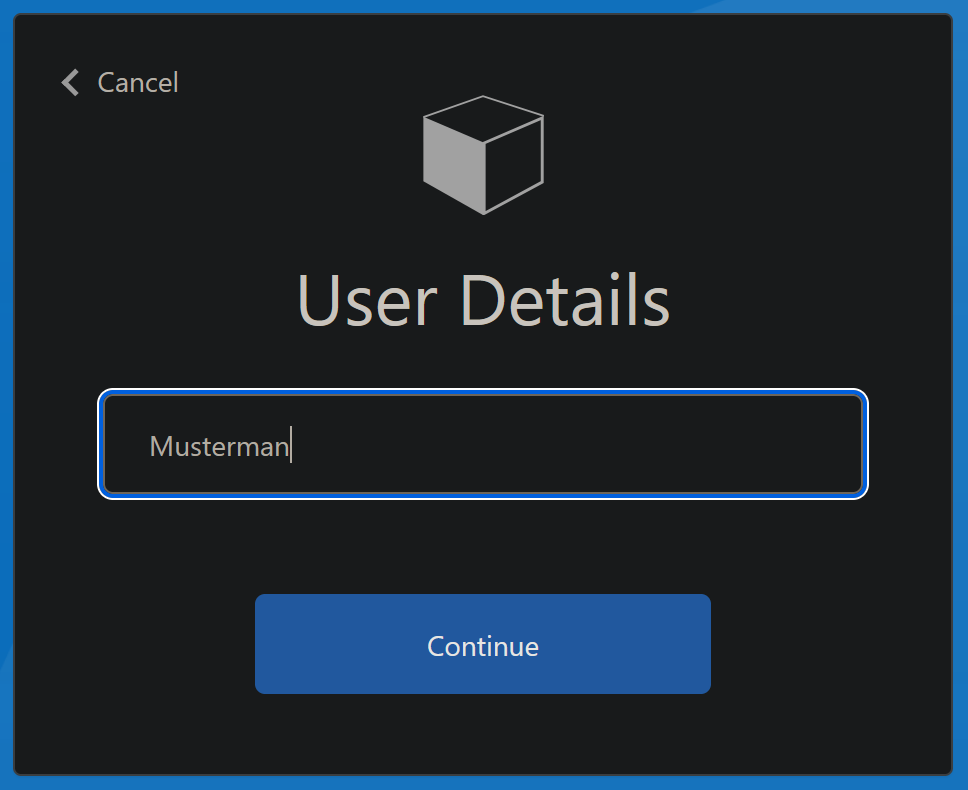
\includegraphics[scale=0.4]{pics/benutzername_aendern.PNG}
    \caption{Benutzername Ändern}
    \label{fig:benutzername-aendern}
\end{figure}

Ein Login-Button ist ebenfalls Bestandteil des Headers. Falls ein Benutzer eingeloggt ist, wird vor dem Login-Button ein zusätzlicher Button angezeigt, der den aktuellen Benutzernamen als Label enthält. Ein Klick auf diesen Button führt zu einer separaten Seite, auf der der Benutzername geändert werden kann.

Die Änderung des Benutzernamens erfolgt durch direktes Bearbeiten eines Textfeldes. Um die Änderung zu übernehmen oder zur vorherigen Seite zurückzukehren, steht ein ``Continue''-Button zur Verfügung. Dieser speichert die Anpassung und leitet den Benutzer wieder auf die Website weiter. Um den vorherigen Benutzernamen jedoch beizubehalten oder zur vorherigen Seite zurückzukehren, steht ein Cancel-Button zur Verfügung. 

Der Header bleibt auf allen, mit Angular entwickelten, Seiten der Anwendung unverändert. Diese Konsistenz gewährleistet eine einheitliche Benutzerführung und erleichtert die Navigation innerhalb der Anwendung.


\subsection{Home - Der Einstieg}

Das Layout der Startseite ist zentriert ausgerichtet. Im oberen Bereich der Seite befindet sich das Logo in gro\ss{}er Darstellung, ergänzt durch den Namen der Diplomarbeit. Direkt darunter wird eine Willkommensnachricht angezeigt (siehe Abbildung \ref{fig:homepage}).

\begin{figure} [h t]
    \centering
    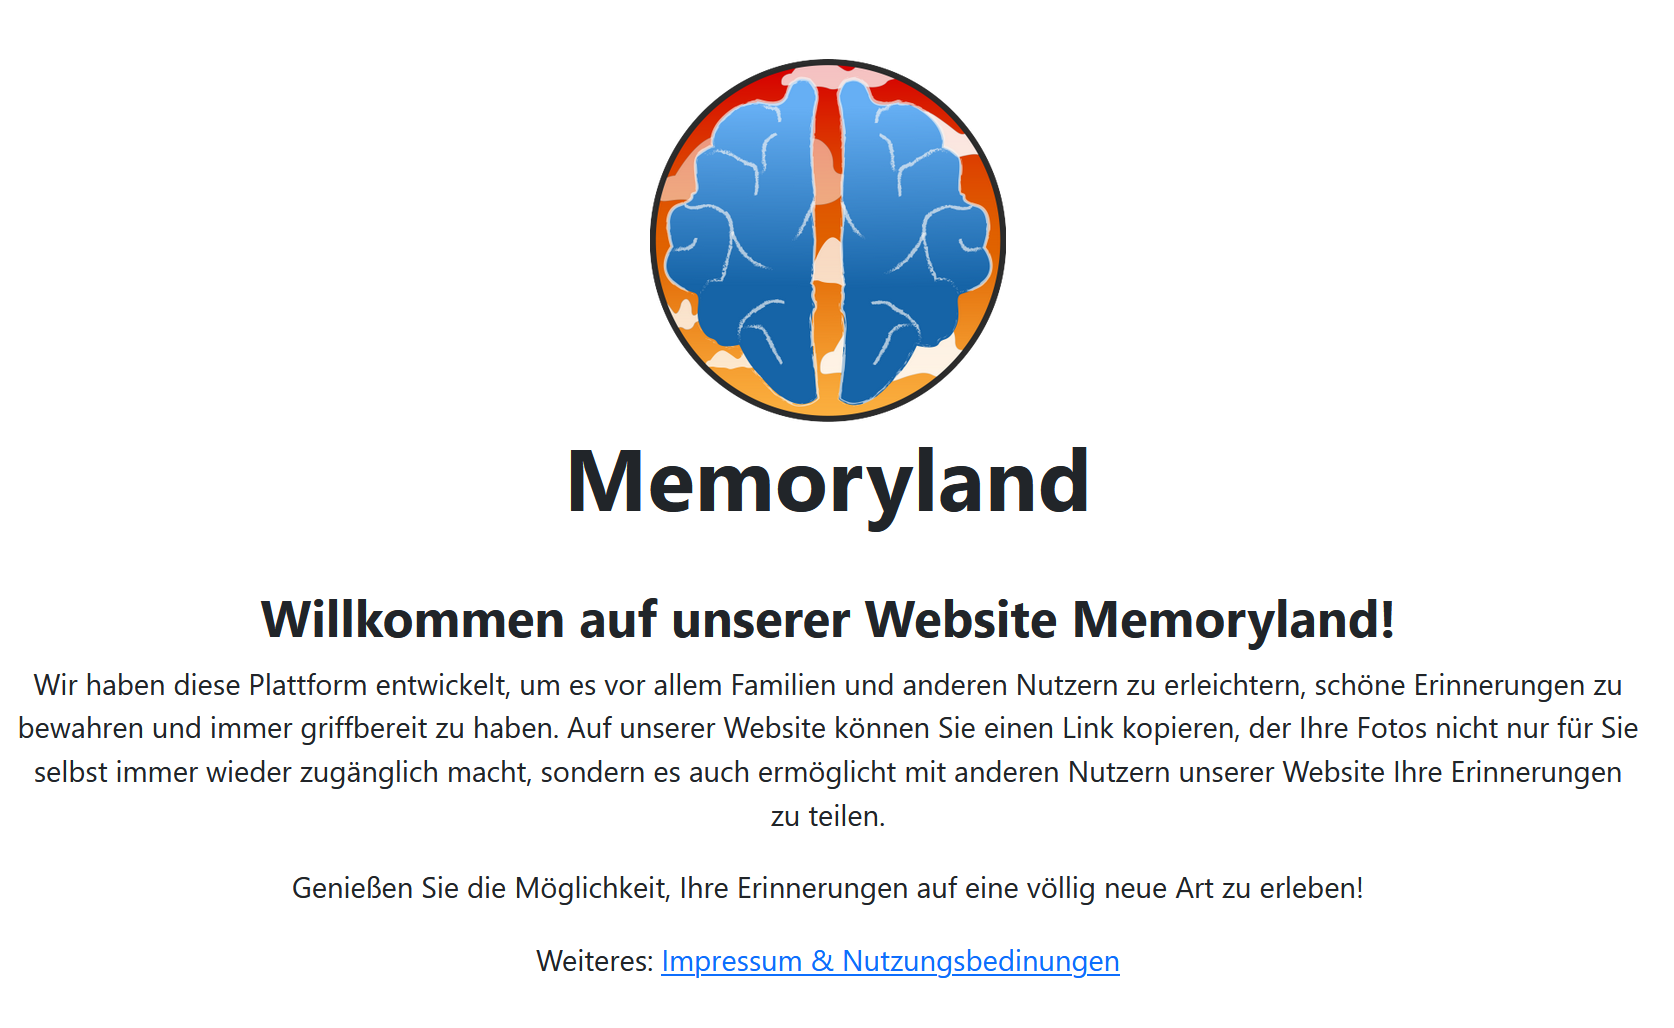
\includegraphics[scale=0.4]{pics/home_page.PNG}
    \caption{Homepage}
    \label{fig:homepage}
\end{figure}


Am unteren Rand der Seite ist ein Link platziert, der zur Impressums- und Nutzungs-bedingungen-Seite führt. Diese Seite ist unter der Sektion ``About'' näher erläutert. Alternativ kann dieselbe Seite über den About-Link im Header aufgerufen werden.

\subsection{About}

Die About-Seite umfasst das Impressum sowie die Nutzungsbedingungen und ist zentriert ausgerichtet.


Das Impressum enthält die Namen der Entwickler und deren Zuständigkeitsbereiche innerhalb der Website, insbesondere die Unterscheidung zwischen Frontend- und Backend-Entwicklung. Zusätzlich sind die vollständige Adresse der Schule mit Stra\ss{}enname, Hausnummer, Postleitzahl, Stadt und Land sowie die offiziellen Kontaktdaten der Schule, einschlie\ss{}lich Telefonnummer und E-Mail-Adresse, aufgeführt.

\begin{figure} [h t]
    \centering
    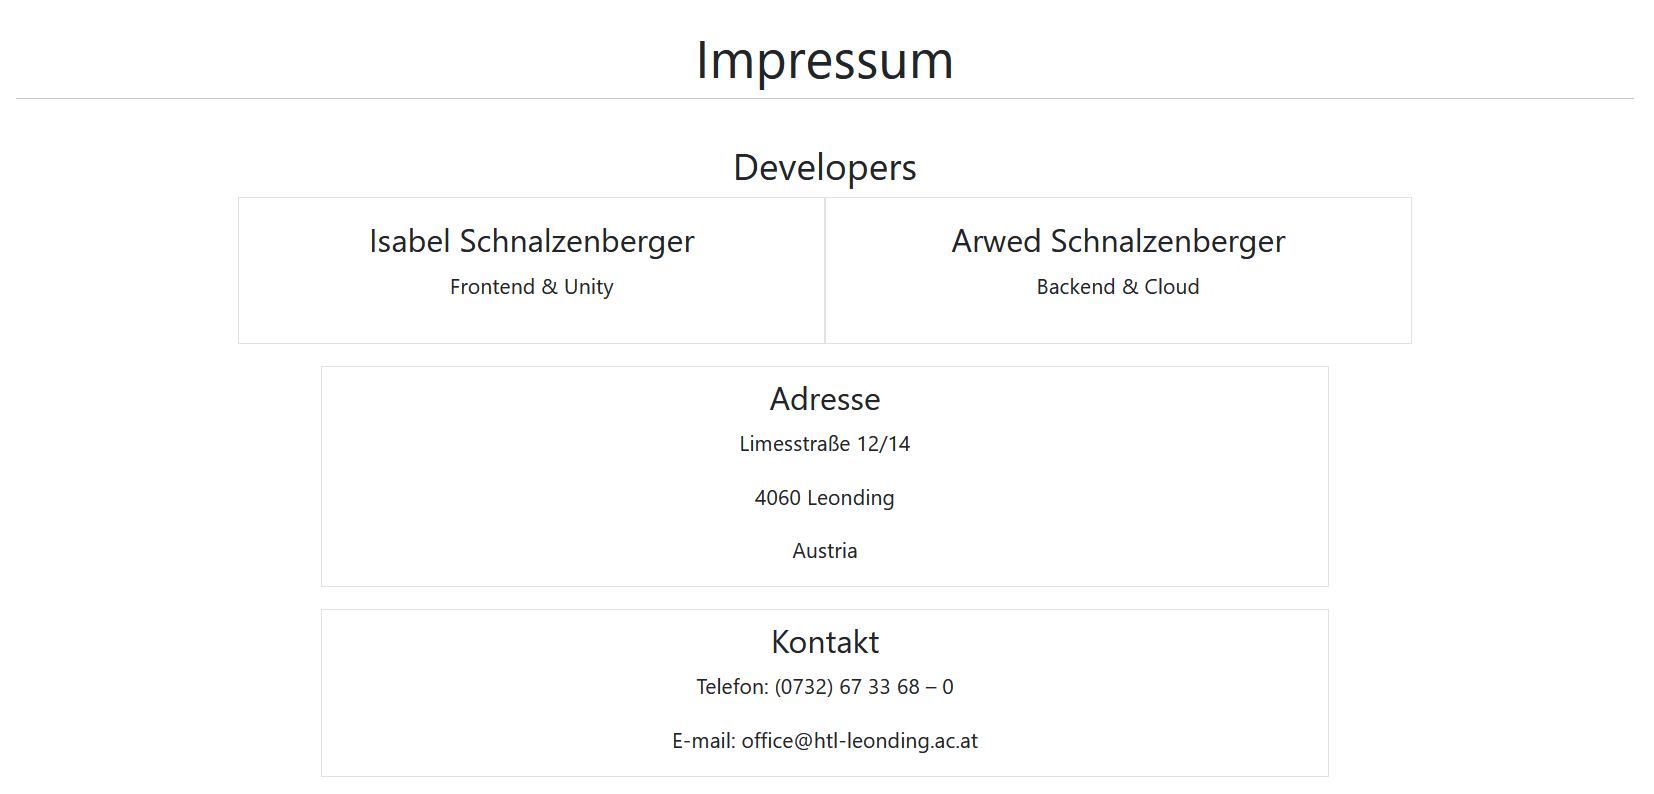
\includegraphics[scale=0.4]{pics/About_page_Impressum.PNG}
    \caption{About - Impressum}
    \label{fig:about-page-impressum}
\end{figure}



\begin{figure} [h t]
    \centering
    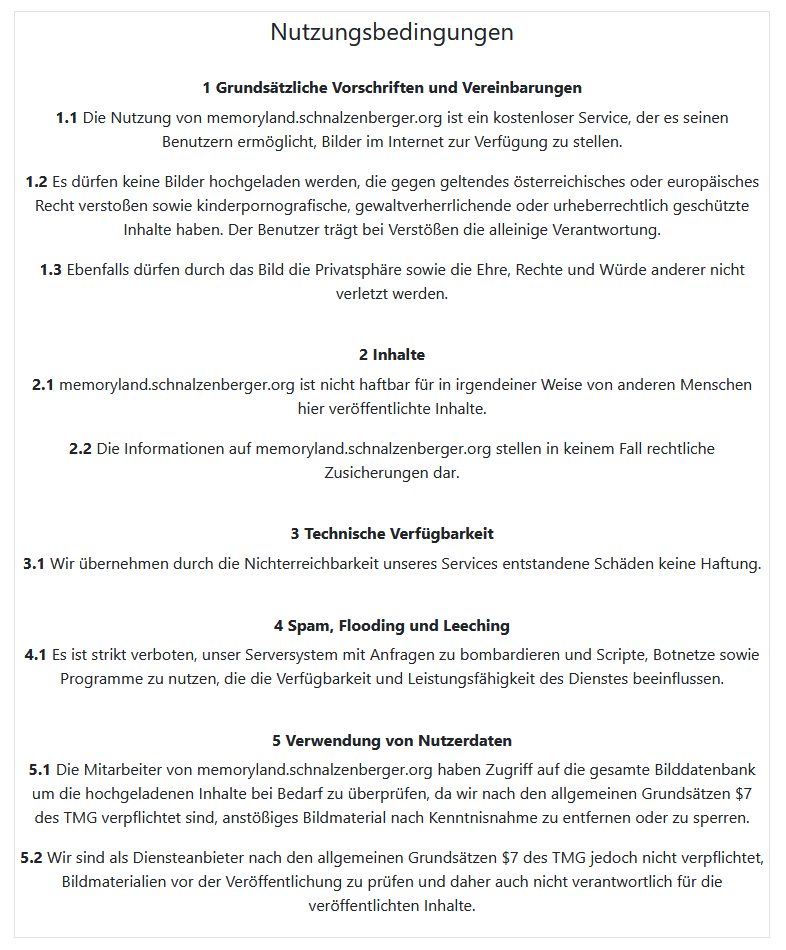
\includegraphics[scale=0.8]{pics/About_page_Nutzungsbedingungen.PNG}
    \caption{About - Nutzungsbedingungen}
    \label{fig:about-page-nutzungsbedingungen}
\end{figure}


Die Nutzungsbedingungen beinhalten allgemeine Vorschriften und Vereinbarungen zur Nutzung der Website. Sie umfassen spezifische Regelungen zu erlaubten und nicht erlaubten Inhalten, die technische Verfügbarkeit der Plattform sowie Bestimmungen zu unerwünschten Aktivitäten wie Spam, Flooding und Leeching. Zudem gibt es eine Sektion zur Verarbeitung und Nutzung von Nutzerdaten, die den Umgang mit personenbezogenen Informationen beschreibt.

Die Betreiber einer Website, wie der hier beschriebenen, müssen sich gegen den missbräuchlichen Umgang und die Verbreitung von verbotenen Materialien schützen. Derartige Nutzungsbedingungen gehören also genauso zum Umfang eines derartigen Projektes wie die Implementierung selbst.






\subsection{Memory Store}

Der Memory Store ist in drei Abschnitte unterteilt und bietet verschiedene Funktionen zur Verwaltung von Fotoalben und Bildern. Die Benutzeroberfläche ist so gestaltet, dass alle wesentlichen Aktionen über interaktive Elemente, wie Buttons und Suchleisten, zugänglich sind.

\subsubsection{Meine Fotoalben - Das Menü}

\begin{wrapfigure}{r}{0.4\textwidth}
    \centering
    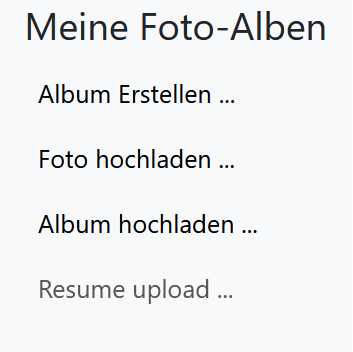
\includegraphics[scale=0.8]{pics/memory_store_menu.PNG}
    \caption{Memory Store Menü}
    \label{fig:memory-store-menu}
\end{wrapfigure}


Dieser Abschnitt enthält mehrere Buttons zur Verwaltung und Organisation von Fotoalben und hochzuladenen Bildern (siehe \ref{fig:memory-store-menu}).

Der erste Button mit der Bezeichnung ``Album Erstellen'' öffnet ein Pop-up-Fenster, in dem der Benutzer den Namen des neuen Albums in ein Textfeld eingeben kann. Falls der Erstellungsprozess abgebrochen werden soll, kann entweder der ``Cancel''-Button oder das Schlie\ss{}symbol (X) oben rechts im Pop-up-Fenster gedrückt werden. Nach der Eingabe des gewünschten Namens wird das Album durch Drücken des ``Album Erstellen''-Buttons endgültig erstellt und der Liste der vorhandenen Alben hinzugefügt.


{\textit{Foto Hochladen}}

Der zweite Button mit der Bezeichnung ``Foto Hochladen'' ermöglicht das Hochladen einzelner Bilder in zuvor erstellte Alben. Nach Betätigung dieses Buttons öffnet sich ein Pop-up-Fenster, in dem zunächst ein Album aus einer Liste bestehender Alben ausgewählt werden muss. Anschlie\ss{}end kann eine Datei vom eigenen Computer durch Drücken des ``Browse''-Buttons ausgewählt werden. Sobald eine Datei ausgewählt wurde, wird ihr Name in einem Textfeld angezeigt. Der Benutzer hat an dieser Stelle die Möglichkeit, den Namen der Datei manuell zu ändern. Das Hochladen des ausgewählten Bildes erfolgt schlie\ss{}lich durch Drücken des ``Foto Hochladen''-Buttons am unteren Rand des Pop-ups (siehe \ref{fig:memory-store-foto-hochladen}).

\begin{wrapfigure}{r}{0.4\textwidth}
    \centering
    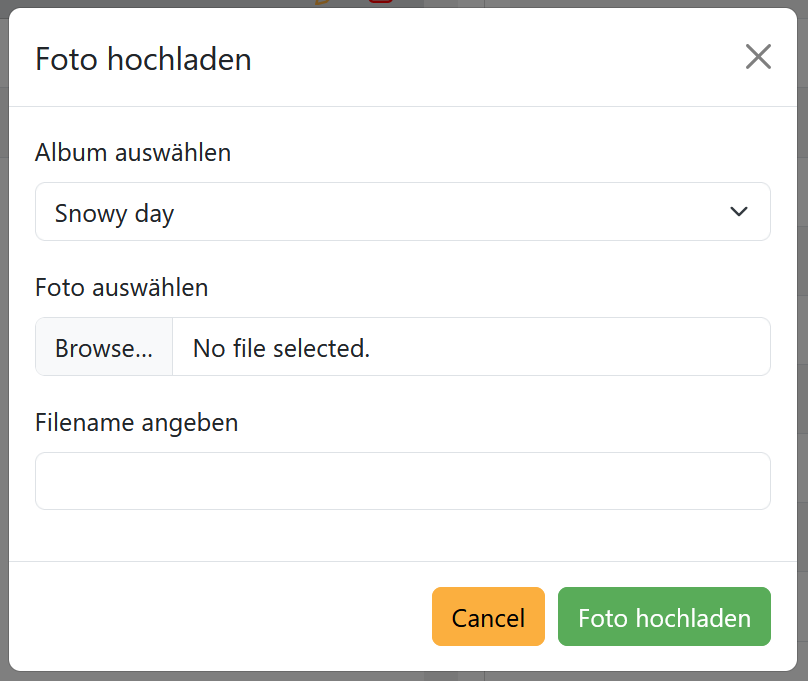
\includegraphics[scale=0.4]{pics/memory_store_teil1_button2.PNG}
    \caption{Memory Store - Foto Hochladen}
    \label{fig:memory-store-foto-hochladen}
\end{wrapfigure}


{\textit{Album Hochladen}}


Der dritte Menüpunkt mit der Bezeichnung ``Album Hochladen'' ermöglicht das Hochladen eines gesamten Albums bzw. eines lokalen Ordners mit mehreren Bildern. Beim Anklicken öffnet sich ein Pop-up-Fenster, in dem zunächst ein Zielalbum aus der Liste zuvor erstellter Alben ausgewählt werden muss. Anschlie\ss{}end kann ein Album vom lokalen Computer über den ``Browse''-Button ausgewählt werden. Nach der Auswahl wird angezeigt, wie viele Bilder sich in dem gewählten Album befinden. Zusätzlich gibt es eine Checkbox, die – falls aktiviert – einen resumable Upload ermöglicht. Diese Funktion erlaubt es, den Upload-Prozess bei einer Unterbrechung fortzusetzen.

\begin{wrapfigure}{r}{0.4\textwidth}
    \centering
    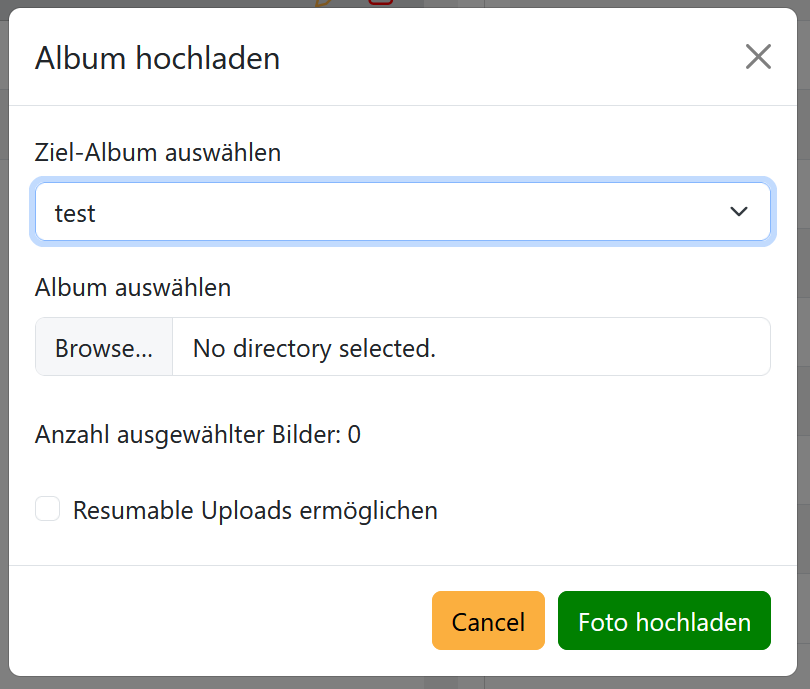
\includegraphics[scale=0.4]{pics/memory_store_teil1_button3.PNG}
    \caption{Memory Store - Album Hochladen}
    \label{fig:memory-store-album-hochladen}
\end{wrapfigure}

Nachdem der Benutzer den ``Fotos Hochladen''-Button betätigt, wird das aktuelle Pop-up-Fenster durch ein neues ersetzt, das eine Fortschrittsanzeige (Progress Bar) enthält. Diese zeigt an, wie viele der Bilder bereits hochgeladen wurden. Sobald der Upload abgeschlossen ist, kann der Vorgang durch Drücken des ``Exit''-Buttons beendet werden.

Falls der Upload während des Prozesses unterbrochen wird, kann er später fortgesetzt werden. Eine Unterbrechung erfolgt entweder durch das Drücken des ``Exit''-Buttons oder durch das Klicken au\ss{}erhalb des Pop-ups. Voraussetzung für die Fortsetzung ist, dass die resumable Upload-Funktion zuvor aktiviert wurde. In diesem Fall kann der Upload über den vierten Button ``Resume Upload'' erneut gestartet werden. Um den Upload fortzusetzen, muss das zuvor ausgewählte Album, von dem die Bilder stammen (footnote siehe discord), erneut ausgewählt werden. Nach der Auswahl kann man den Upload weiterführen. Während sich ein Upload im gestoppten Zustand befindet, ist das Hochladen weiterer Alben nicht möglich bis der laufende Upload abgeschlossen wurde.

\subsubsection{Alben}

Dieser Abschnitt enthält eine Suchleiste, mit der der Benutzer nach einem bestimmten Album suchen kann. Während der Eingabe von Zeichen oder Wörtern werden, automatisch alle Alben angezeigt, die den eingegebenen Begriff enthalten. Diese Echtzeit-Suche erleichtert die Navigation innerhalb der gespeicherten Alben.

\begin{wrapfigure}{r}{0.4\textwidth}
    \centering
    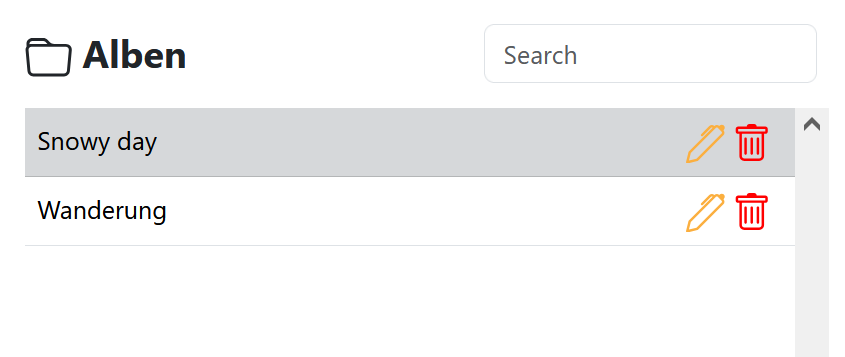
\includegraphics[scale=0.5]{pics/memory_store_teil2.PNG}
    \caption{Memory Store - Alben}
    \label{fig:memory-store-alben}
\end{wrapfigure}

Direkt unter der Suchleiste befindet sich eine Liste aller vom Benutzer erstellten Alben. Jedes Album wird mit seinem Namen angezeigt und hat zwei interaktive Symbole neben sich.

Das Stift-Symbol ermöglicht das Umbenennen des Albums. Durch Klicken auf das Symbol öffnet sich ein Pop-up-Fenster mit einem Textfeld, in das der neue Name eingegeben und bestätigt werden kann.

Das Papierkorb-Symbol ermöglicht das Löschen des Albums. Sobald der Button gedrückt wird, wird das Album ohne weitere Bestätigung gelöscht. Alle darin gespeicherten Fotos werden damit ebenfalls entfernt.

Falls ein Album durch Anklicken ausgewählt wird, erscheint sein Inhalt im dritten Abschnitt, der die enthaltenen Fotos anzeigt.

\subsubsection{Fotos}

\begin{figure} [h t]
    \centering
    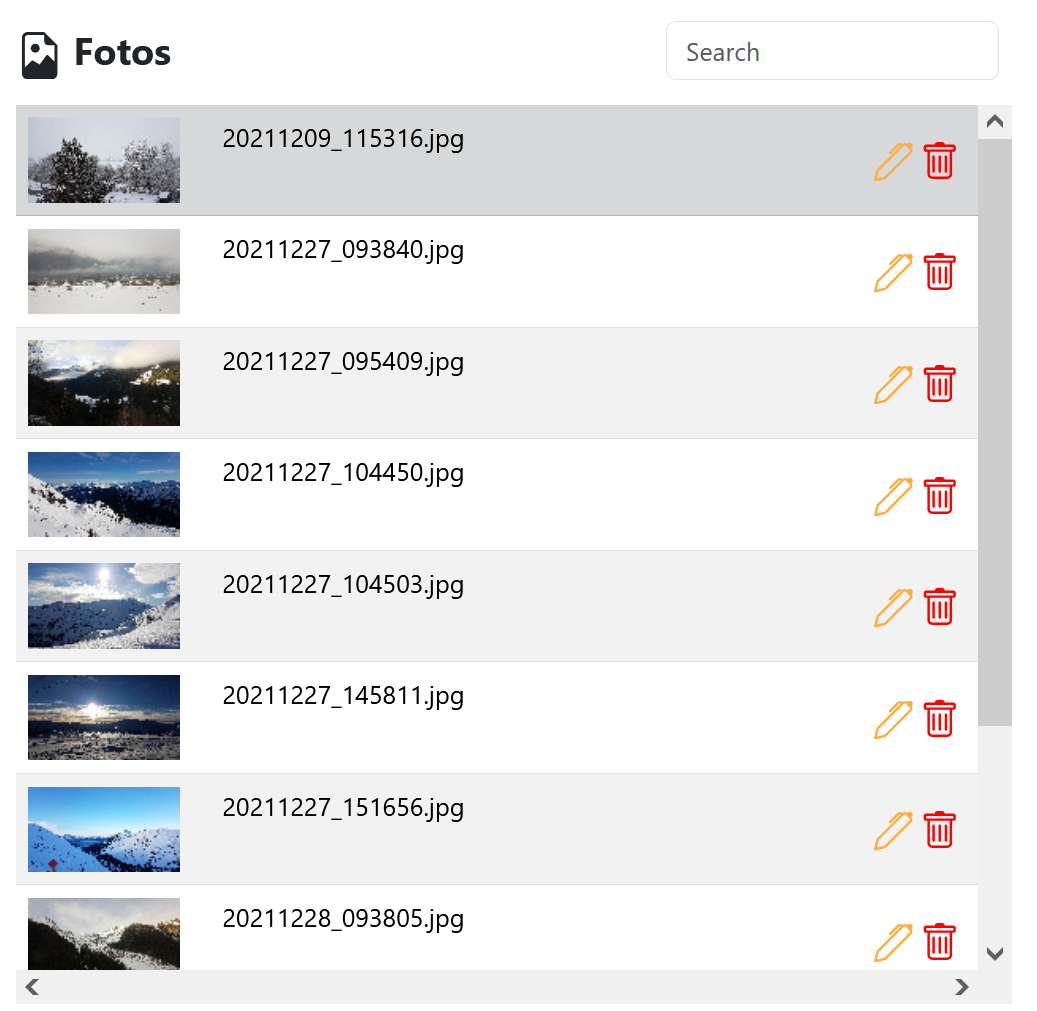
\includegraphics[scale=0.7]{pics/memory_store_teil3.PNG}
    \caption{Memory Store - Fotos}
    \label{fig:memory-store-fotos}
\end{figure}

Im oberen Bereich befindet sich eine Suchleiste, die identisch zur Suchfunktion in Abschnitt 2 arbeitet. Hier kann der Benutzer gezielt nach bestimmten Fotos innerhalb des gewählten Albums suchen.

Wenn kein Album in Abschnitt ``Alben'' ausgewählt wurde, bleibt dieser Bereich leer. Sobald jedoch ein Album ausgewählt wurde, werden die darin enthaltenen Fotos im unteren Bereich inklusive kleiner Vorschaubilder aufgelistet.

Jedes Foto wird mit seinem Namen angezeigt und besitzt zwei interaktive Symbole direkt daneben.

Das Stift-Symbol ermöglicht das Umbenennen des Bildes. Durch Anklicken wird ein Textfeld geöffnet, in das der neue Name eingetragen werden kann.

Das Papierkorb-Symbol löscht das Foto dauerhaft. Das Bild wird nach Betätigung des Symbols ohne weitere Bestätigung aus dem Album entfernt.

Falls ein Foto durch Anklicken ausgewählt wird, öffnet sich eine Ansicht mit dem Bild, in der der Dateiname zusätzlich angezeigt wird. 

\subsection{All Worlds}

\begin{wrapfigure}{r}{0.4\textwidth}
    \centering
    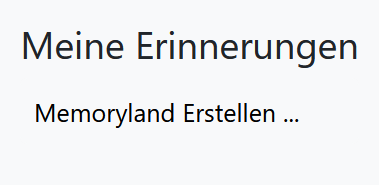
\includegraphics[scale=0.7]{pics/all_worlds_teil1.PNG}
    \caption{All Worlds - Menü}
    \label{fig:all-worlds-menu}
\end{wrapfigure}

Die Erstellung und Verwaltung von Memorylands erfolgt ausschlie\ss{}lich auf der Seite ``All Worlds''. Diese Seite ist in zwei Hauptabschnitte unterteilt, die unterschiedliche Funktionen bieten.

\clearpage

\subsubsection{Meine Erinnerungen}


\begin{wrapfigure}{r}{0.4\textwidth}
    \centering
    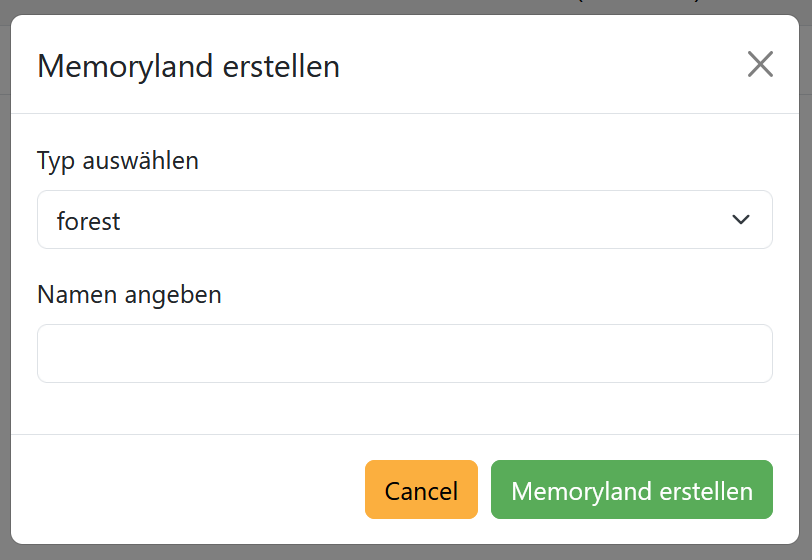
\includegraphics[scale=0.5]{pics/all_worlds_teil1_button.PNG}
    \caption{Memoryland erstellen}
    \label{fig:all-worlds-memoryland-erstellen}
\end{wrapfigure}

Der erste Abschnitt trägt die Bezeichnung ``Meine Erinnerungen''. Hier befindet sich ein Button mit der Aufschrift ``Memoryland Erstellen''. Durch das Anklicken dieses Buttons wird ein Pop-up-Fenster geöffnet, in dem verschiedene Einstellungen für das neue Memoryland vorgenommen werden können. Es enthält eine Auswahlmöglichkeit, in der der gewünschte Typ des Memorylands bestimmt werden kann. Zur Verfügung stehen zwei verschiedene Typen: ``Forest'' und ``Island''. Diese Typen definieren die visuelle Darstellung der Bilder innerhalb des Memorylands. Zusätzlich ist ein Textfeld vorhanden, in das der gewünschte Name des Memorylands eingetragen werden kann.



\subsubsection{Memorylands}

Der zweite Abschnitt der Seite trägt den Namen ``Memorylands'' und dient der Verwaltung bereits erstellter Memorylands. Um ein bestimmtes Memoryland schnell zu finden, steht eine Suchleiste zur Verfügung. Durch das Eintippen eines Namens oder einzelner Zeichen werden bereits während der Eingabe passende Ergebnisse gefiltert und angezeigt. Direkt unterhalb dieser Suchleiste werden alle zuvor erstellten Memorylands in einer trukturierten Übersicht dargestellt. Jedes Memoryland wird dabei mit mehreren Informationen versehen. Dazu gehören der Name des Memorylands, der gewählte Typ sowie die maximale Anzahl an Fotos, die innerhalb dieses Memorylands gespeichert werden können. Zusätzlich befinden sich neben diesen Informationen drei verschiedene Symbole, die für die Bearbeitung und Verwaltung der Memorylands vorgesehen sind.

\begin{figure} [h t]
    \centering
    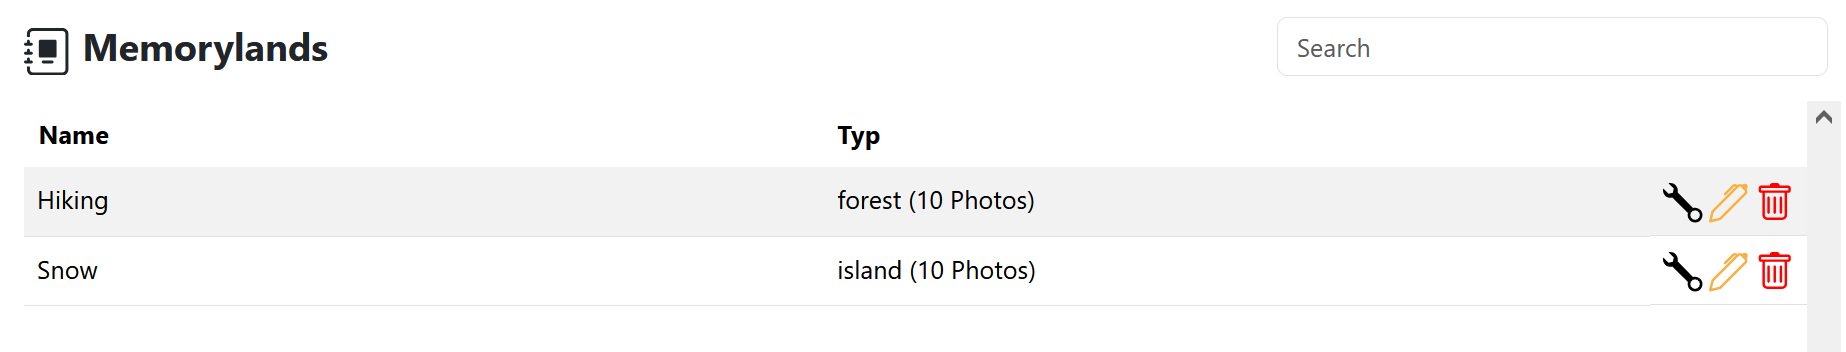
\includegraphics[scale=0.6]{pics/all_worlds_teil2.PNG}
    \caption{Memorylands Übersicht}
    \label{fig:all-worlds-memorylands}
\end{figure}

Das mittlere Symbol ist ein Stift-Icon. Durch das Anklicken dieses Symbols wird die Möglichkeit geboten, den Namen des Memorylands zu ändern. Ein Eingabefeld erscheint, in das ein neuer Name eingetragen werden kann. Das nächste Symbol ist ein Papierkorb-Icon. Wenn dieses Symbol betätigt wird, wird das Memoryland unwiderruflich gelöscht. Eine zusätzliche Sicherheitsabfrage erfolgt dabei nicht, sodass das Memoryland sofort aus der Liste entfernt wird. 

Das forderste Symbol ist ein Schraubenschlüssel-Icon. Durch das Anklicken dieses Symbols öffnet sich ein weiteres Pop-up-Fenster, das zusätzliche Bearbeitungsoptionen bereitstellt. 

\subsubsection{Memorylands editieren}

In diesem Pop-up-Fenster kann ein bestehendes Fotoalbum aus der eigenen Sammlung ausgewählt werden, aus dem Bilder in das Memoryland eingefügt werden sollen. Um Bilder in das Memoryland zu integrieren, steht eine Drag-and-Drop-Funktion zur Verfügung. 

\begin{figure} [h t]
    \centering
    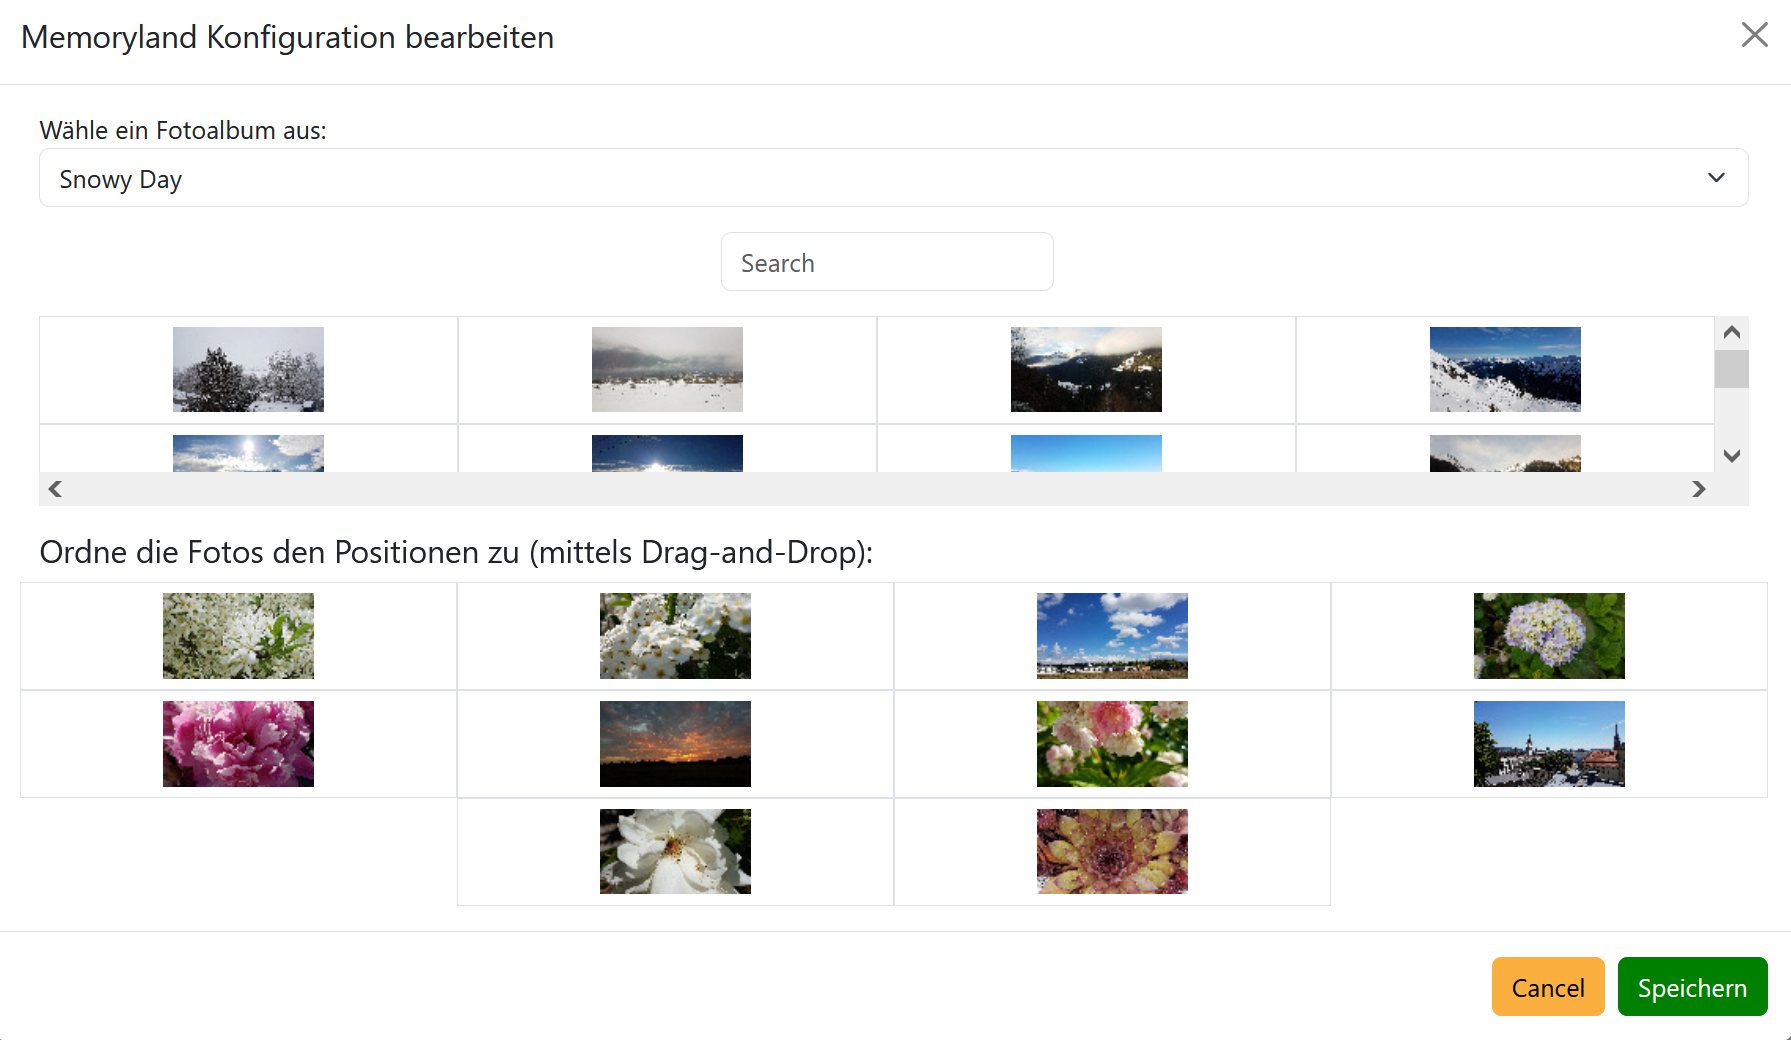
\includegraphics[scale=0.6]{pics/all_worlds_teil2_button.PNG}
    \caption{Memorylands editieren}
    \label{fig:all-worlds-memorylands-editieren}
\end{figure}

Bilder können aus einem oberen Bereich des Fensters in einen unteren Bereich verschoben werden. Falls sich eine gro\ss{}e Anzahl an Bildern in dem ausgewählten Album befindet, kann eine zusätzliche Suchleiste genutzt werden, um gezielt nach bestimmten Bildern zu suchen.

\clearpage

\subsection{Explore Worlds}
\label{subsec:frontend-explore-worlds}

\begin{figure} [h t]
    \centering
    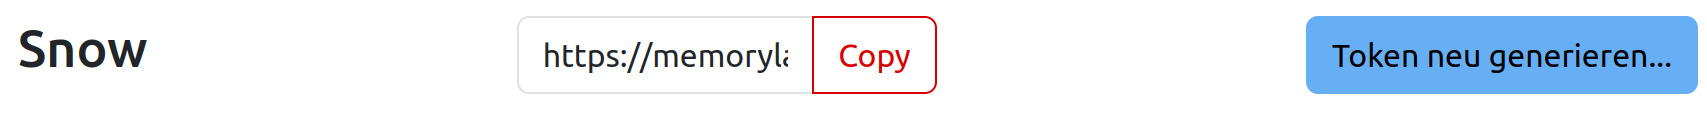
\includegraphics[scale=0.2]{pics/explore_worlds_header.png}
    \caption{Explore Worlds - Zugang}
    \label{fig:explore-worlds-overview}
\end{figure}

Nachdem ein Memoryland erfolgreich erstellt wurde, kann es über die Übersicht in \textbf{``All Worlds''} aufgerufen werden. Sobald der Nutzer auf den Namen eines Memoryland klickt, erfolgt eine automatische Weiterleitung zur Seite ``Explore Worlds''. Dort wird das ausgewählte Memoryland sofort geladen und visuell dargestellt. Dies ermöglicht eine interaktive Betrachtung der gespeicherten Erinnerungen innerhalb der gewählten Umgebung.

Abbildung \ref{fig:explore-worlds-overview} zeigt den oberen Bereich des Fensters. Diese stellt zwei Funktionen zur Verfügung: Den \textbf{Token}\footnote{siehe dazu vor allem auch den Abschnitt \ref{backend-memoryland-controller}}-Link  und einen Button um einen Token neu zu generieren.

\begin{figure} [h t]
    \centering
    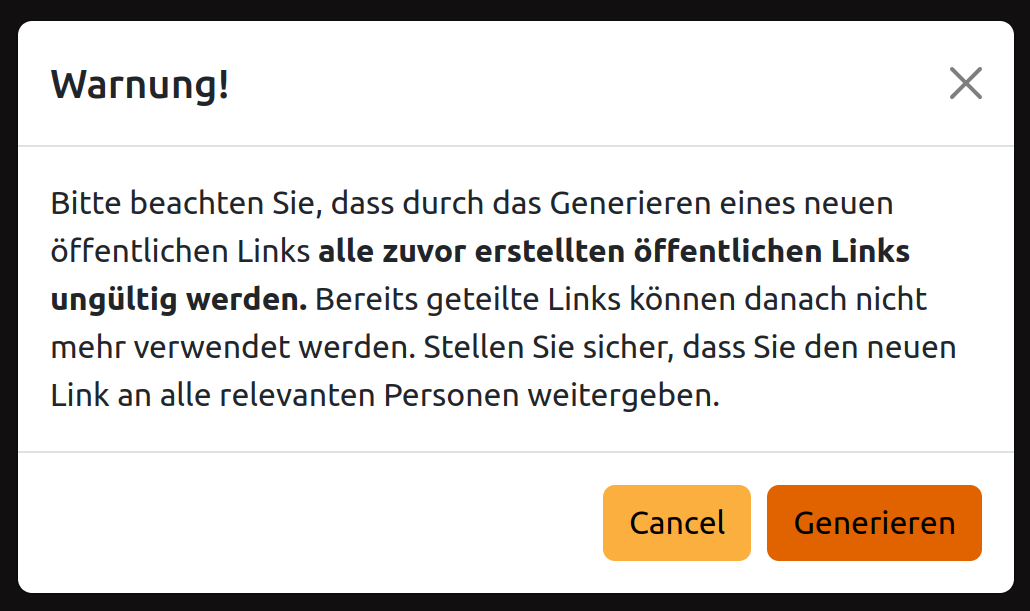
\includegraphics[scale=0.35]{pics/explore-worlds-warning.png}
    \caption{Explore Worlds - Warnung über Ungültigkeit bisheriger Links}
    \label{fig:explore-worlds-warning}
\end{figure}

Der Button \emph{erneuert den Token} für das gewählte bzw. angezeigte Memoryland. Diese Prozedur hat zwei Effekte: der alte Token und damit alle bisher geteilten Links werden für dieses Memoryland ungültig und ein neues Token wird generiert und im Token-Link Element angezeigt. Um den Benutzer explizit auf die dann wirkende \emph{Ungültigkeit der bisherigen Links} der alten, vielleicht bereits verteilten Links zu erinnern wird kurz die Information in Abbildung \ref{fig:explore-worlds-warning} angezeigt.

\begin{figure} [h t]
    \centering
    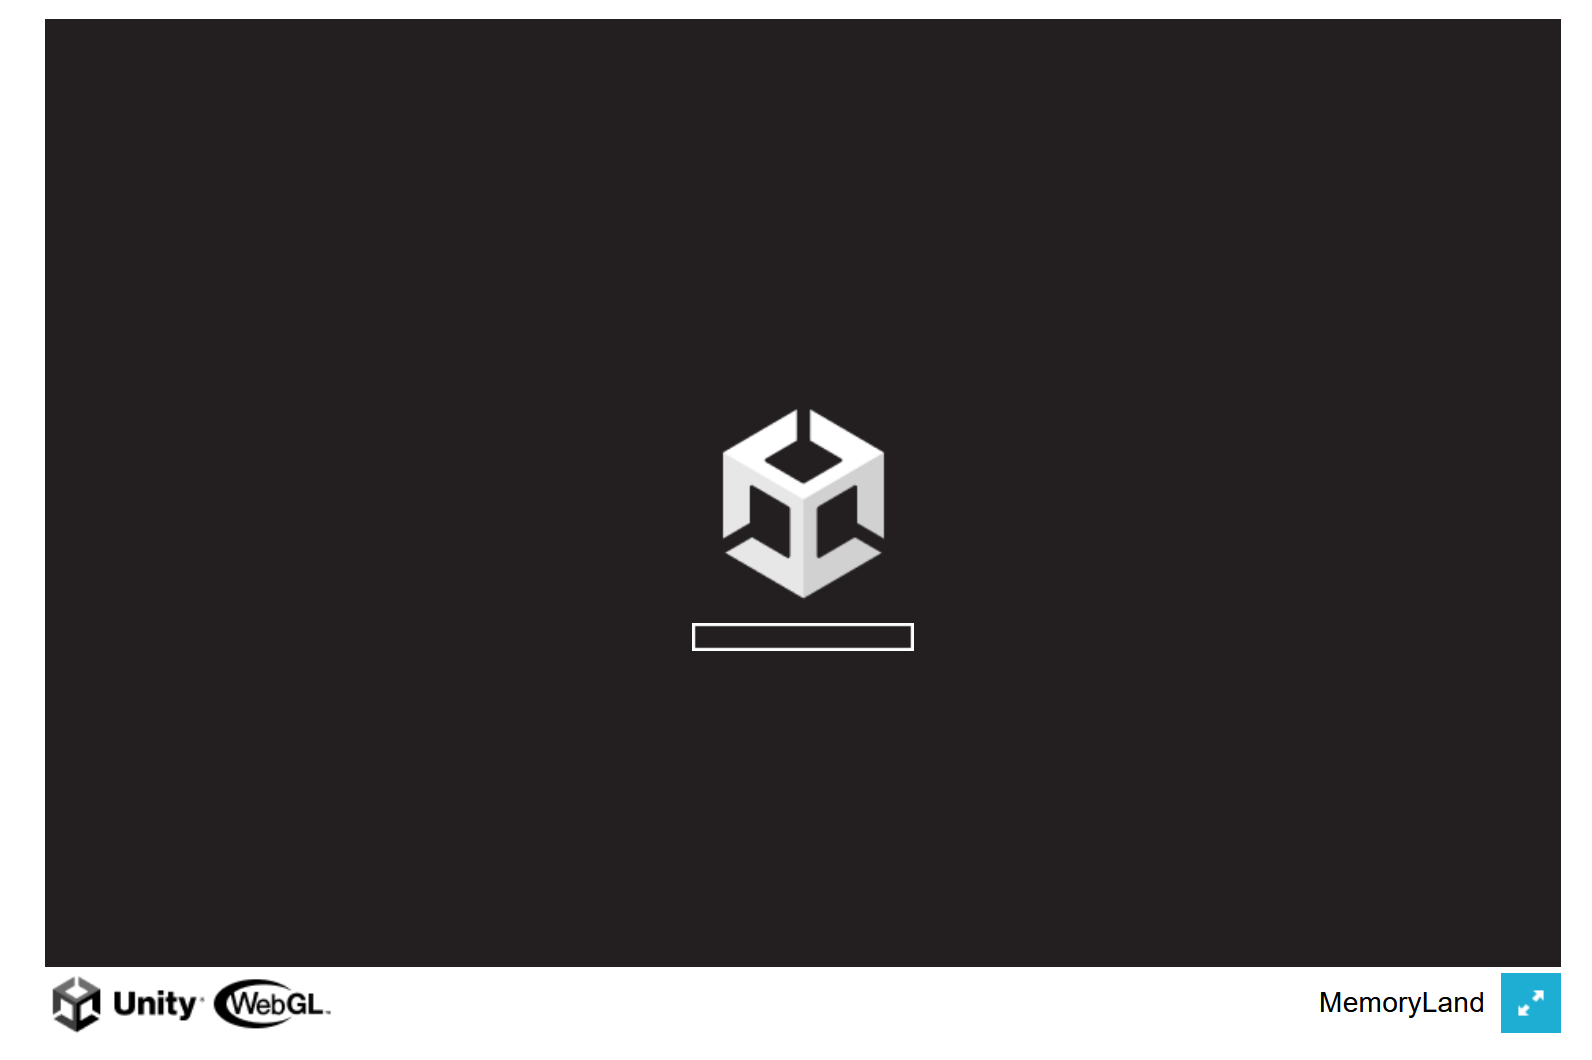
\includegraphics[scale=0.5]{pics/explore_worlds_loading_unity.PNG}
    \caption{Explore Worlds - Unity wird geladen}
    \label{fig:explore-worlds-loading-unity}
\end{figure}

Wenn nun eine Memoryland \textbf{World (Szene)} geladen wird, muss zuerst Unity geladen werden. Dazu zeigt die Unity WebGL folgende Animation in Abbildung \ref{fig:explore-worlds-loading-unity}. Die Beladung wurde zeitoptimiert, zusätzliche Einstellung zu Caching wurden im Build mitgegeben. Leider funktionieren diese in den aktuellen Unity Versionen nicht und die Entwickler hoffen, dass dies mit neueren Versionen behoben wird.\footnote{siehe hierzu Abschnitt \ref{sec:unity-webgl} bzw. auch Quellen hierzu \cite{UnityDocsDataCachingIssue} und \cite{UnityDocsDataCachingIssue2}}


\begin{figure} [h t]
    \centering
    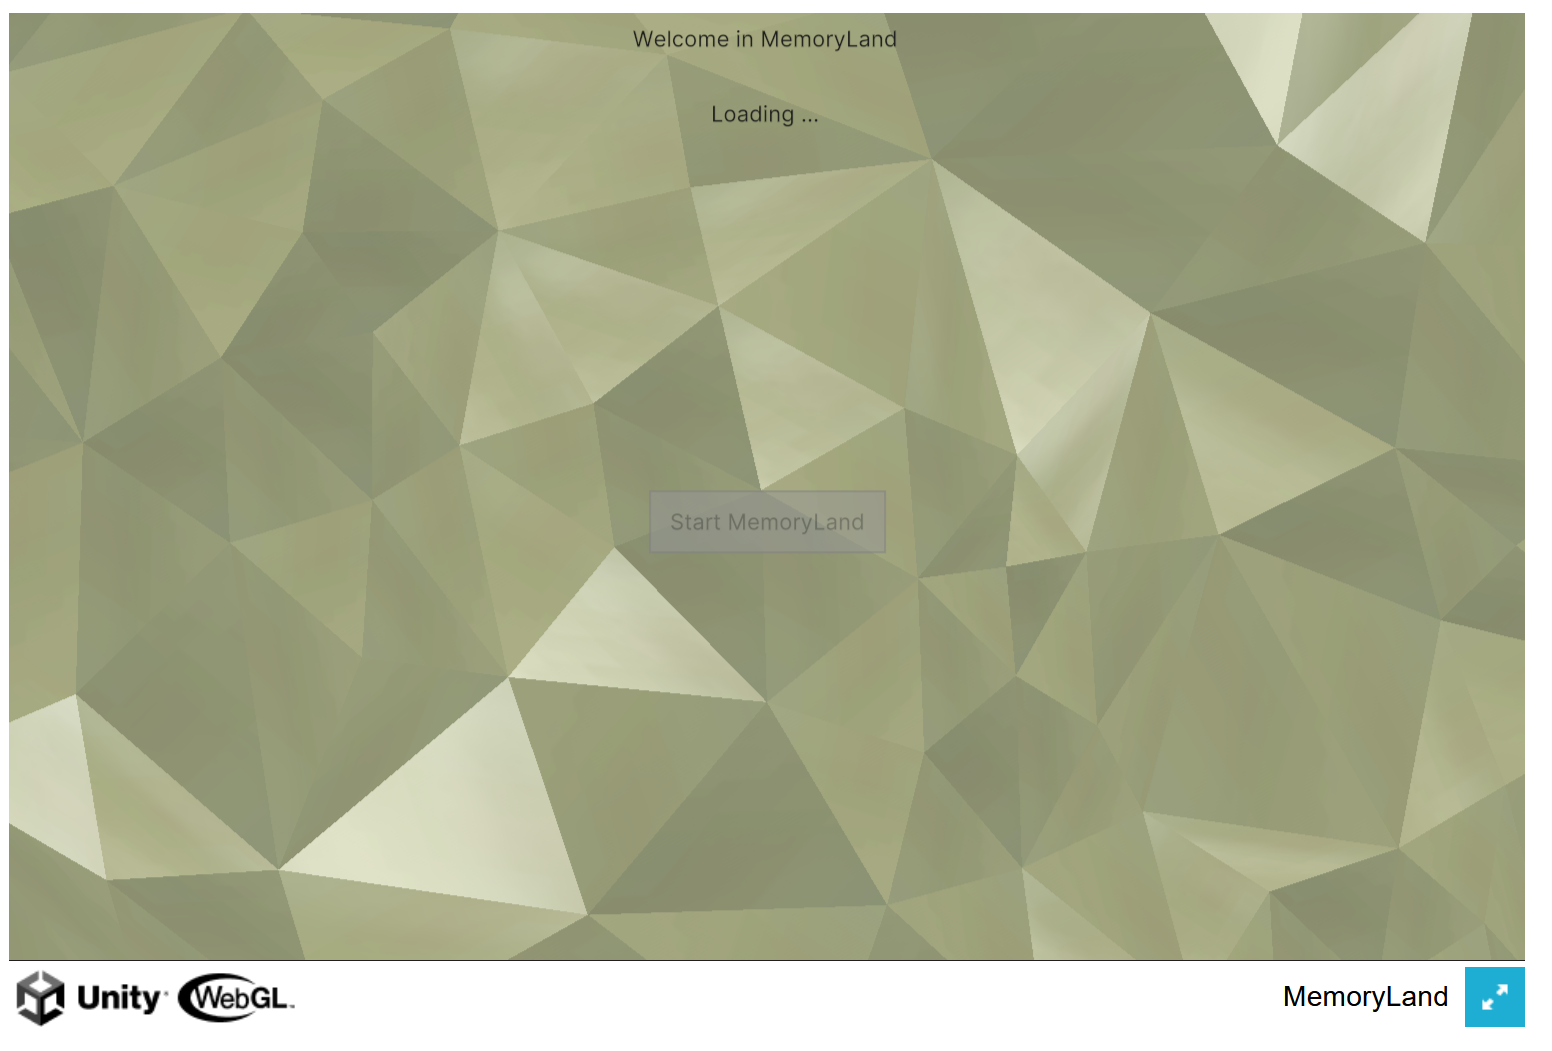
\includegraphics[scale=0.5]{pics/explore_worlds_loading.PNG}
    \caption{Explore Worlds - Bilder werden geladen}
    \label{fig:explore-worlds-loading}
\end{figure}


Danach startet die Unity Applikation (siehe Abbildung 
\ref{fig:explore-worlds-loading}) von Memoryland und lädt die World (Szene) vom Backend. Dazu muss zuerst die Szenenart (MemorylandType) und die gewählten Bilder im Backend aufbereitet werden. Die Bilder werden mit SAS-Tokens\footnote{siehe vor allem \ref{subsection:sas-token-generation} und \ref{subsection:azure-blob-storage-getting-started}} als URLs vom Backend zur Verfügung gestellt und dann über das Azure Storage geladen. Das Laden \footnote{siehe vor allem Abschnitt \ref{subsec:unity-startup-scene}} erfolgt aus Verzerrungs- und Zeitgründen vorab. Die Bilder sind dann zum Zeitpunkt des Starts des immersiven Erlebnisses bereits vollständig vorhanden und der Benutzer kann das Erlebnis ohne Probleme genie\ss{}en. 


\begin{figure} [h t]
    \centering
    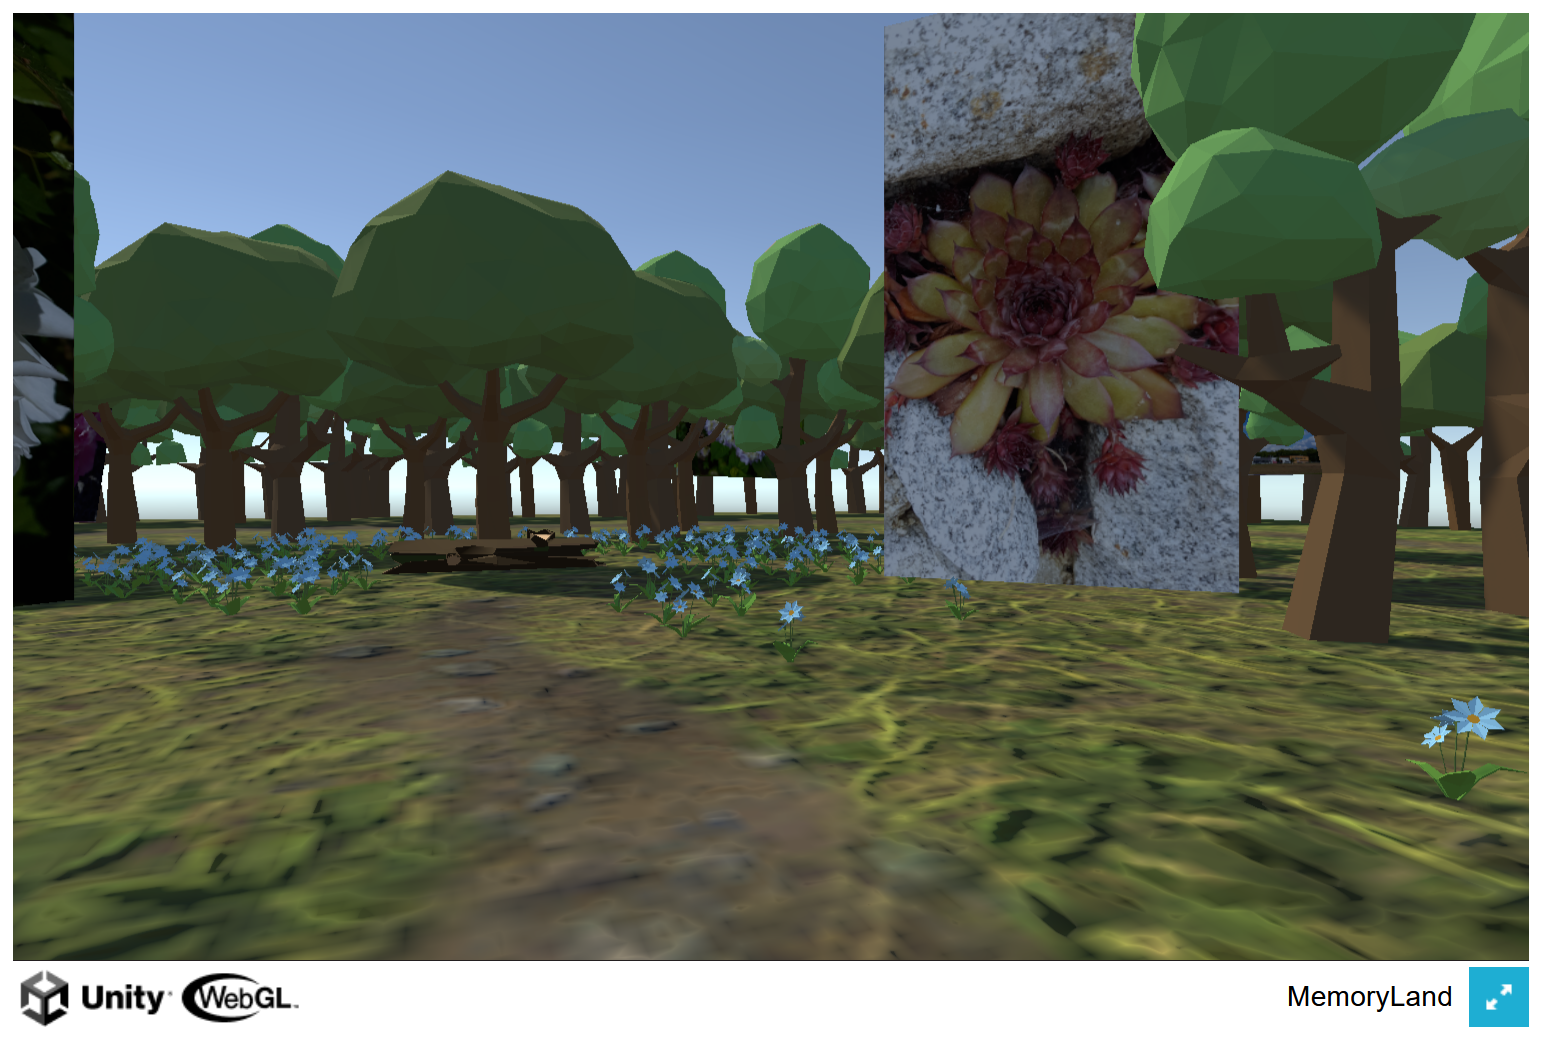
\includegraphics[scale=0.5]{pics/explore_worlds_forest.PNG}
    \caption{Explore Worlds - Eine Wald-Szene}
    \label{fig:explore-worlds-forest}
\end{figure}

Am Ende steht nun einem \textbf{angemeldeten} genauso wie einem \textbf{unangemeldeten Benutzer} (über den zuvor erhaltenen Link mit Token) das \textbf{immersive Erlebnis} eines Memoryland zur Verfügung. Die Abbildung \ref{fig:explore-worlds-forest} zeigt den Durchlauf einer Wald Szene. Diese enthält, genauso wie die zweite zu Beginn der Entwicklung gewählte Insel-Szene, bis zu zehn Bilder. 

\begin{figure} [h t]
    \centering
    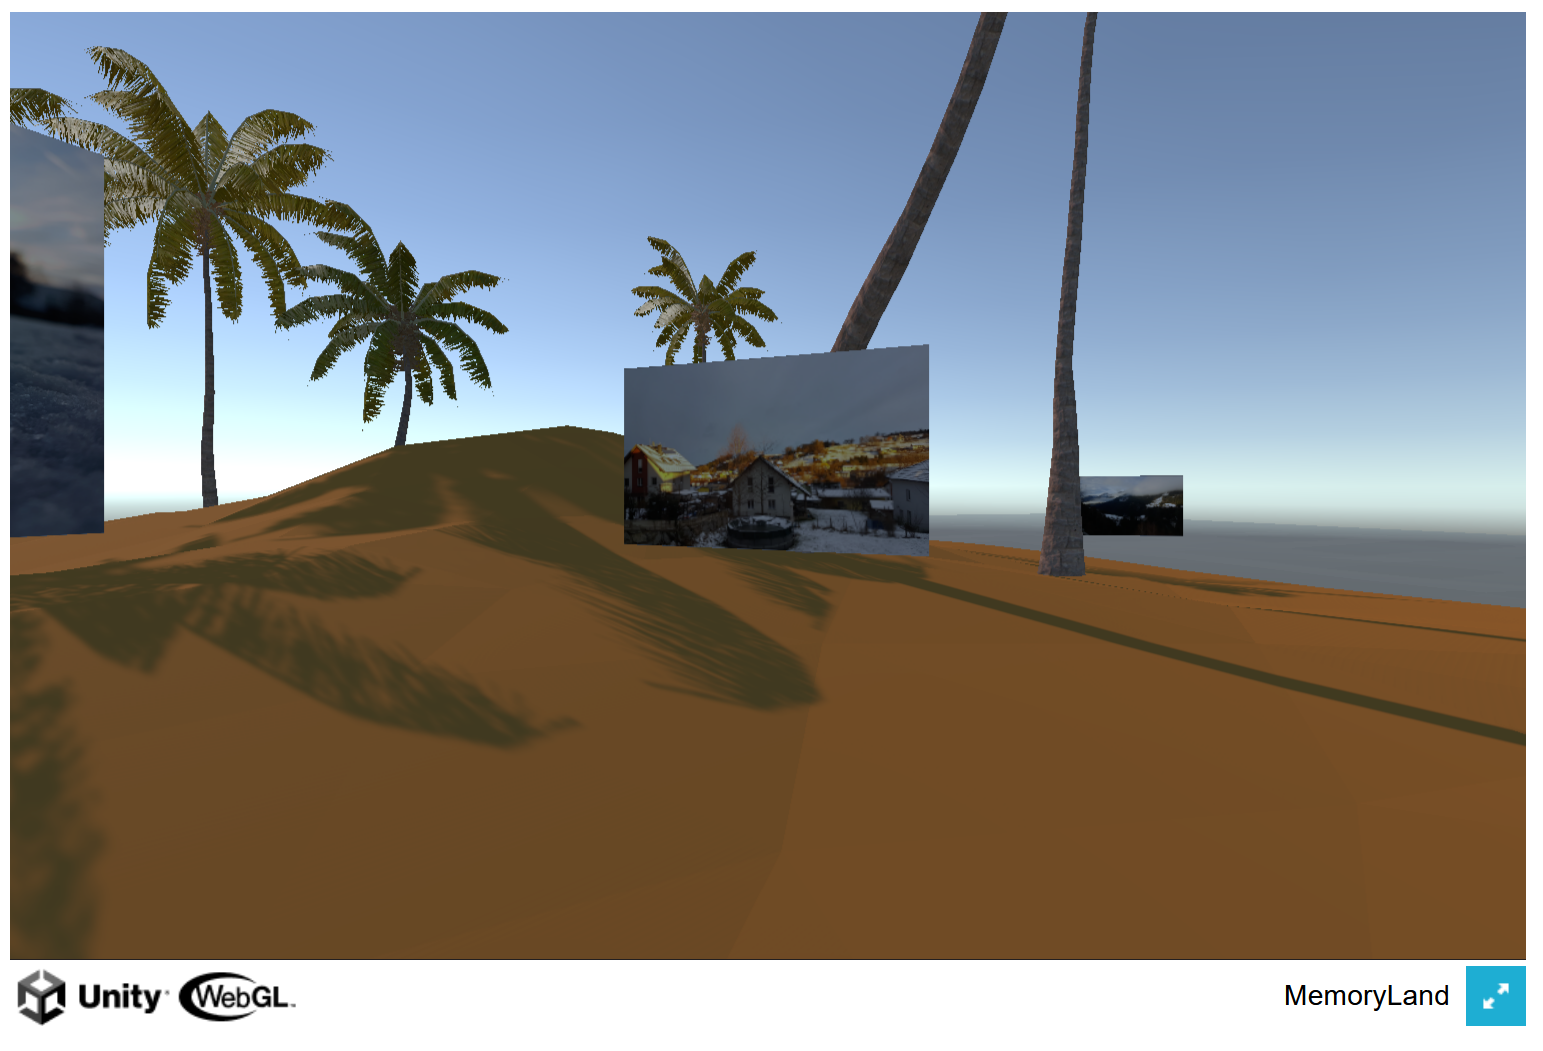
\includegraphics[scale=0.5]{pics/explore_worlds_island.PNG}
    \caption{Explore Worlds - Eine Insel-Szene}
    \label{fig:explore-worlds-island}
\end{figure}



Das zweite zur Verfügung stehende Memoryland ist die Insel-Szene. Sie findet auf einer sandigen Insel mit Palmen am Stand statt. Man überschreitet die Insel und kann sich die zehn gewählten Bilder in Ruhe ansehen. Abbildung \ref{fig:explore-worlds-island} zeigt den Durchlauf einer solchen Szene.


\subsection{Toasts}

\textbf{Toasts} sind eine \textbf{visuelle Rückmeldung} für Benutzer und zeigen an, ob eine Aktion erfolgreich war, fehlgeschlagen ist oder allgemeine Informationen enthält.  

Die Toast-Nachrichten erscheinen im oberen rechten Bereich der Website, jedoch unterhalb des Headers. Sie bleiben für eine bestimmte Zeit sichtbar und verschwinden automatisch. Alternativ können sie durch das Klicken auf ein ``X''-Symbol manuell geschlossen werden.  

Es gibt drei verschiedene \textbf{Farbvarianten}, die jeweils eine spezifische Bedeutung haben. Ein \textbf{grüner Toast} signalisiert ``Success'' und zeigt an, dass eine Aktion erfolgreich abgeschlossen wurde, beispielsweise die Erstellung eines Albums oder eines Memorylands. Ein \textbf{roter Toast} steht für ``Error'' und bedeutet, dass während eines Prozesses ein Fehler aufgetreten ist, wodurch der Vorgang unterbrochen oder gestoppt wurde. Ein \textbf{blauer Toast} steht für ``Information'' und enthält eine neutrale Nachricht, die lediglich eine Mitteilung darstellt, ohne dass es sich um eine Erfolgsmeldung oder eine Fehlermeldung handelt.


Durch die Farbkennzeichnung wird die Bedeutung der Toast-Nachricht sofort erkennbar. Dies verbessert die Benutzerfreundlichkeit, da Informationen schnell erfasst werden 
können, ohne dass zusätzliche Interaktionen erforderlich sind.



